The CLAS12 detector \figref{fig:clas12photo} has two major subsystems: the Forward Detector and the Central Detector, as well as a forward tagger (nested inside the forward detector package) and backward angle neutron detector (BAND). 



\begin{figure}[H]
    \centering
    \subfloat[CLAS12 CAD layout.]{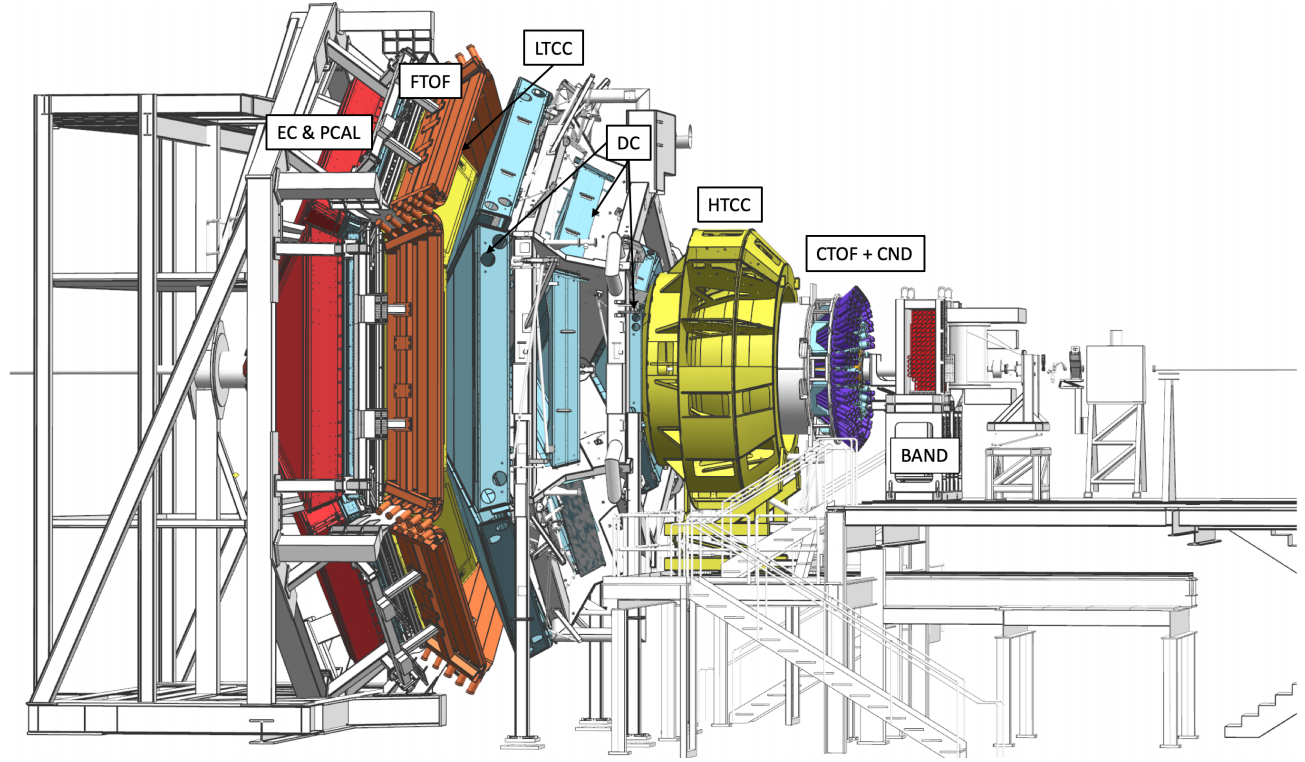
\includegraphics[width=0.45\textwidth]{Chapters/Ch2-Experiment/clas-12-exp/clas-detectors/other/pics/CLAS12.png}\label{fig:clas12}}
    \hfill
    \subfloat[CLAS12, fully installed.]{\includegraphics[width=0.45\textwidth]{Chapters/Ch2-Experiment/clas-12-exp/clas-detectors/other/pics/clas-real.png}\label{fig:clas12spec}}
    \caption[CLAS12 Layout]{CLAS12 layout schematic and photograph, from \parencite{Burkert2020TheLaboratory}.}\label{fig:clas12photo}
\end{figure}



\subsubsection*{Forward Detector}

    The Forward Detector (FD) is a 6-fold azimuthally symmetric segmented system containing several detector packages and a toroidal magnet. The sections follow a counterclockwise numbering convention where S1 corresponds to $[-30^{\circ}, 30^{\circ}]$, as in \figref{fig:fd_sections}. Working from the target downstream, the FD consists of a High Threshold Cherenkov Counter (HTCC) \parencite{Sharabian2020TheCounter}, Low Threshold Cherenkov Counter (LTCC) \parencite{Ungaro2020TheDetector}, the Ring Imaging Cherenkov detector (RICH) \parencite{Contalbrigo2020TheDetector}, Forward Time-of-Flight (FTOF) \parencite{Carman2020TheSystem}, Drift Chambers (DC) \parencite{Mestayer2020TheSystem} embedded in a 3.5 Tesla torodial magnetic field \parencite{Fair2020TheMagnets}, and Electromagnetic Calorimeter (ECal) complex \parencite{Asryan2020TheCalorimeter}.

    The ECal consists of three layers, two of which are from the previous CLAS experiment \parencite{Amarian2001TheCalorimeter}. Those two layers were only sufficient to contain showers with energies below 5 GeV, so a third layer (Pre-shower Calorimeter, PCal) was added to address this issue, as well as introduce the finer grained segmentation necessary to resolve the angle between the two photons of a neutral pion decay, which is of special importance for this process measurement. The FD system covers approximately $5^{\circ}$ to $35^{\circ}$ in polar angle, with one layer of the FTOF (FTOF-2) extending coverage to $45^{\circ}$. 
    
    %Likewise, the FTOF has three layers---FTOF 1a, FTOF 1b, and FTOF 2. The LTCC and the RICH were not used in this measurement.
               
    \begin{figure}[H]
        \centering
        \subfloat[FD sectioning.]{
            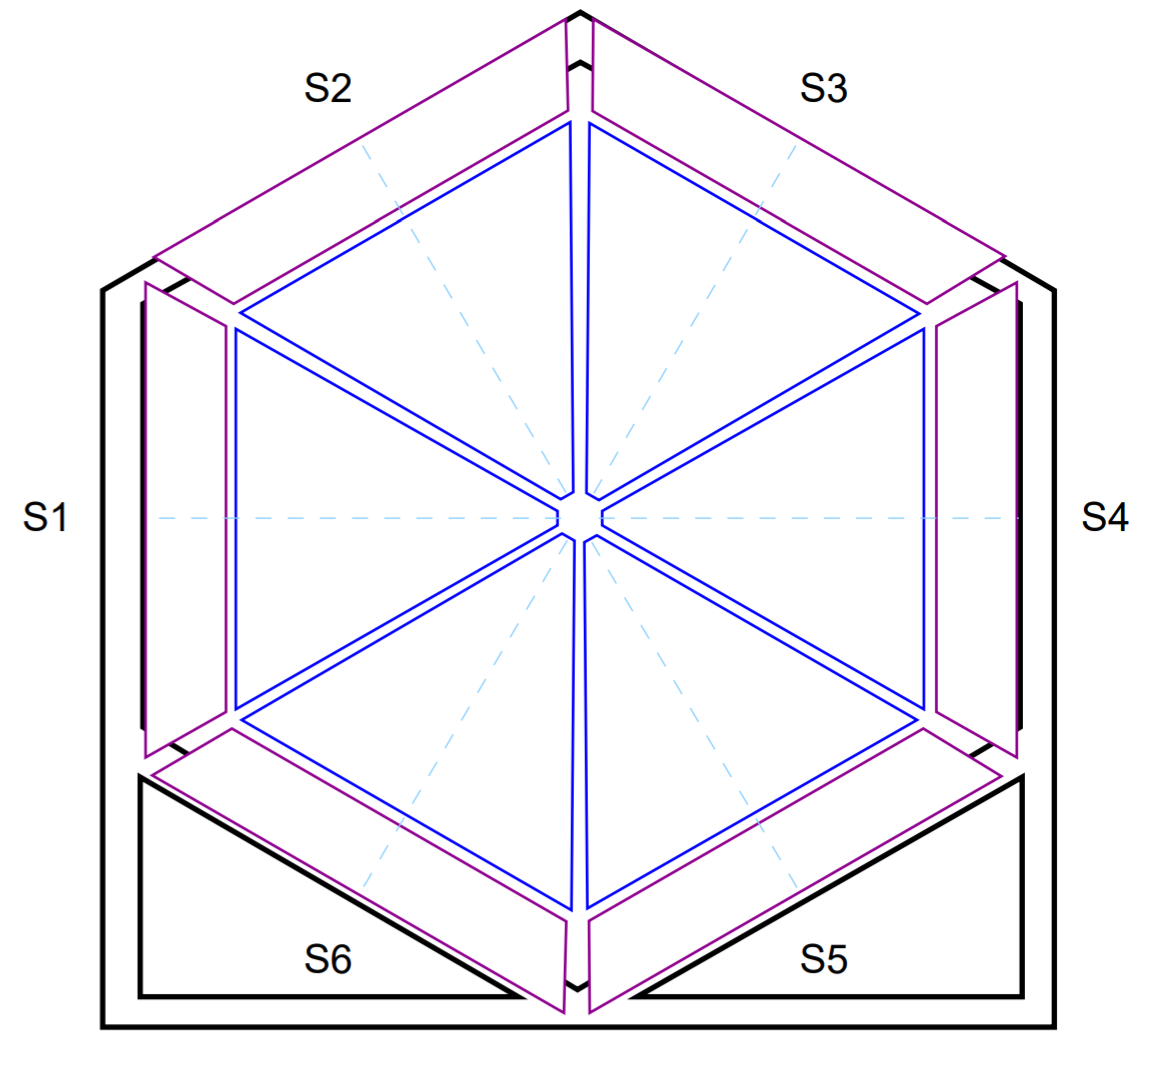
\includegraphics[width=0.3\textwidth]{Chapters/Ch2-Experiment/clas-12-exp/clas-detectors/fd/pics/ftof-front.png}\label{fig:fd_sections}
        }
        \hfill
        \subfloat[Model of HTCC.]{
            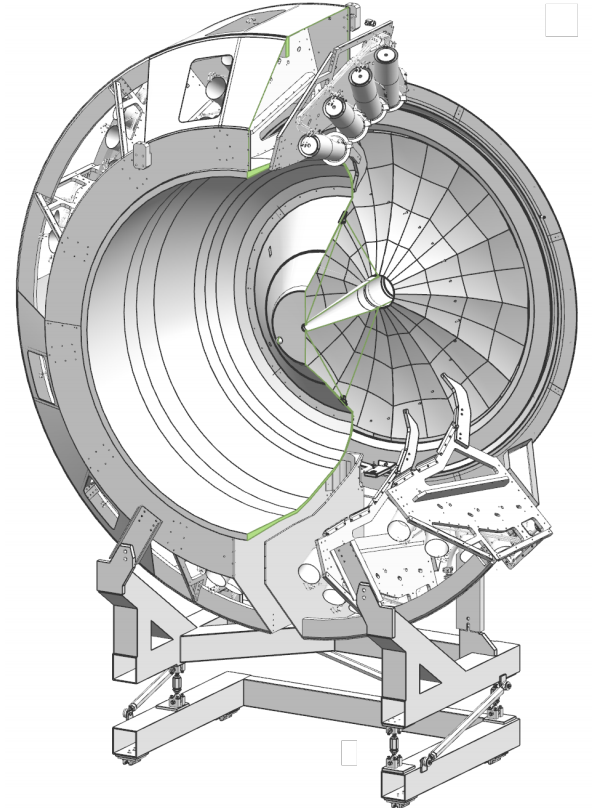
\includegraphics[width=0.3\textwidth]{Chapters/Ch2-Experiment/clas-12-exp/clas-detectors/fd/pics/htcc.png}\label{fig:htcc}
        }
        \hfill
         \subfloat[PCal and ECal assembly.]{
            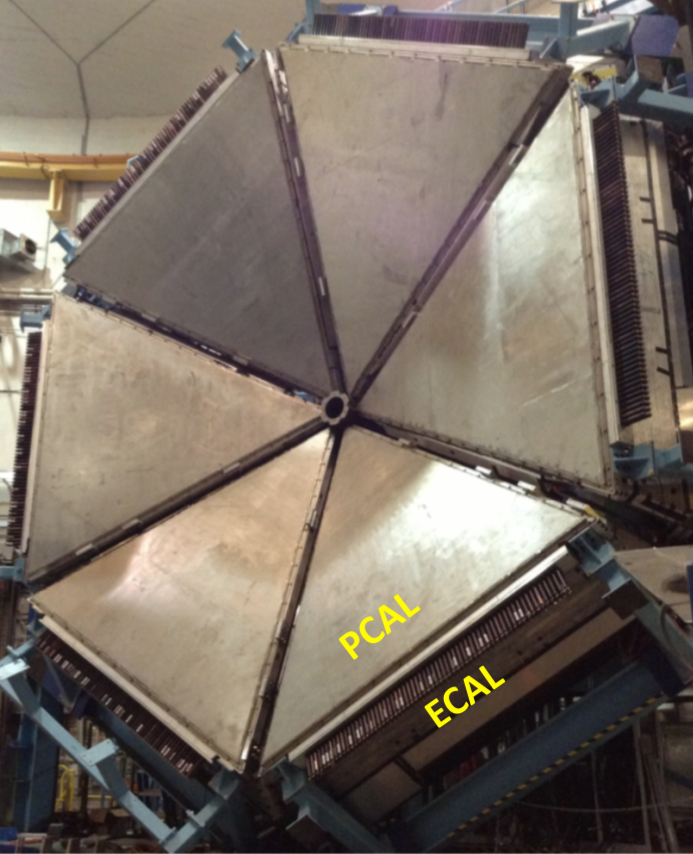
\includegraphics[width=0.3\textwidth]{Chapters/Ch2-Experiment/clas-12-exp/clas-detectors/fd/pics/clas12-pcal-ecal.png}\label{fig:pcalecal}
        }
        \caption[Forward Detector Packages]{The FD is broken into six sections (a), with the exception of the first component after the target, the HTCC (b). The PCal was added to the ECal from the CLAS experiment to achieve the necessary particle resolution. From \parencite{Burkert2020TheLaboratory}}
        \label{fig:select_FD_components}
    \end{figure}




\subsubsection*{Central Detector}

    The Central Detector (CD) also provides nearly 2$\pi$ azimuthal coverage, and spans from $\sim$ $35^{\circ}$  to $125^{\circ}$ in polar angle. The CD is an approximately 1 meter long cylinder inside a 5 Tesla solenoidal magnet \parencite{Fair2020TheMagnets} with four sub-detector packages. From the target working out, the packages are a Central Vertex Tracker \figref{fig:mvt}, made of a Barrel Micromegas Tracker (BMT) \parencite{Acker2020TheTracker} and Silicon Vertex Tracker (SVT) \parencite{Antonioli2020TheTracker}, a Central Time-of-Flight (CTOF) \parencite{Carman2020TheSystem} \ref{fig:ctof}, and a Central Neutron Detector (CND) \parencite{Chatagnon2020TheDetector}, which was installed but not used in this measurement. 
    
    %The main part is the SVT, while the BMT is used to improve the track reconstruction. 

    Low momentum transfer t events correspond to large proton polar angles, meaning the majority of low-t events occur with a proton detected in the CD. These events are important as the GPD interpretation of deeply virtual processes is only valid in the regime where $\frac{-t}{Q^2}$ is small, and as such the CD is invaluable to acquiring data to gain insight on these distributions.        


        %CTOF
        %    Central for PID purposes. Divides into 48 1 meter long plastic scintillators with double sided PMT readout.PMTs are in the 0.1 T fringe field region and enclosed in magnetic shielding. 65 picosecond timing resolution. 35 to 125 degrees, 2 $\pi$ in polar angle. 3 cm x 3 cm scintillator planks. Pion/Kaon separation up to 0.64 GeV, Kaon/proton separation up to 1 GeV, pion proton separation up to 1.25 GeV.  	

 
        
        %Solenoid
	%	    5 Tesla super conducting magnet, uniform field ($\Delta$B/B = $10^-4$). Weakest at small angles, strongest at large angles. Opening polar angle of 40 degrees. Momentum range of interest 0.3 to 1.3 GeV. 18 Megajoules stored energy. 85 cm in diameter, 4.2 Kelvin operation. 


        \begin{figure}[H]
            \centering
            \subfloat[Model of CTOF.]{
                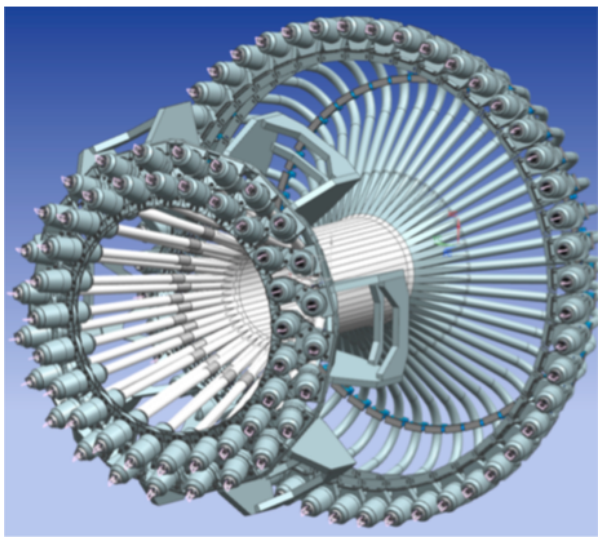
\includegraphics[width=0.3\textwidth]{Chapters/Ch2-Experiment/clas-12-exp/clas-detectors/cd/pics/CTOF.png}\label{fig:ctof}
            }
            \hfill
            \subfloat[Schematic of CVT.]{
                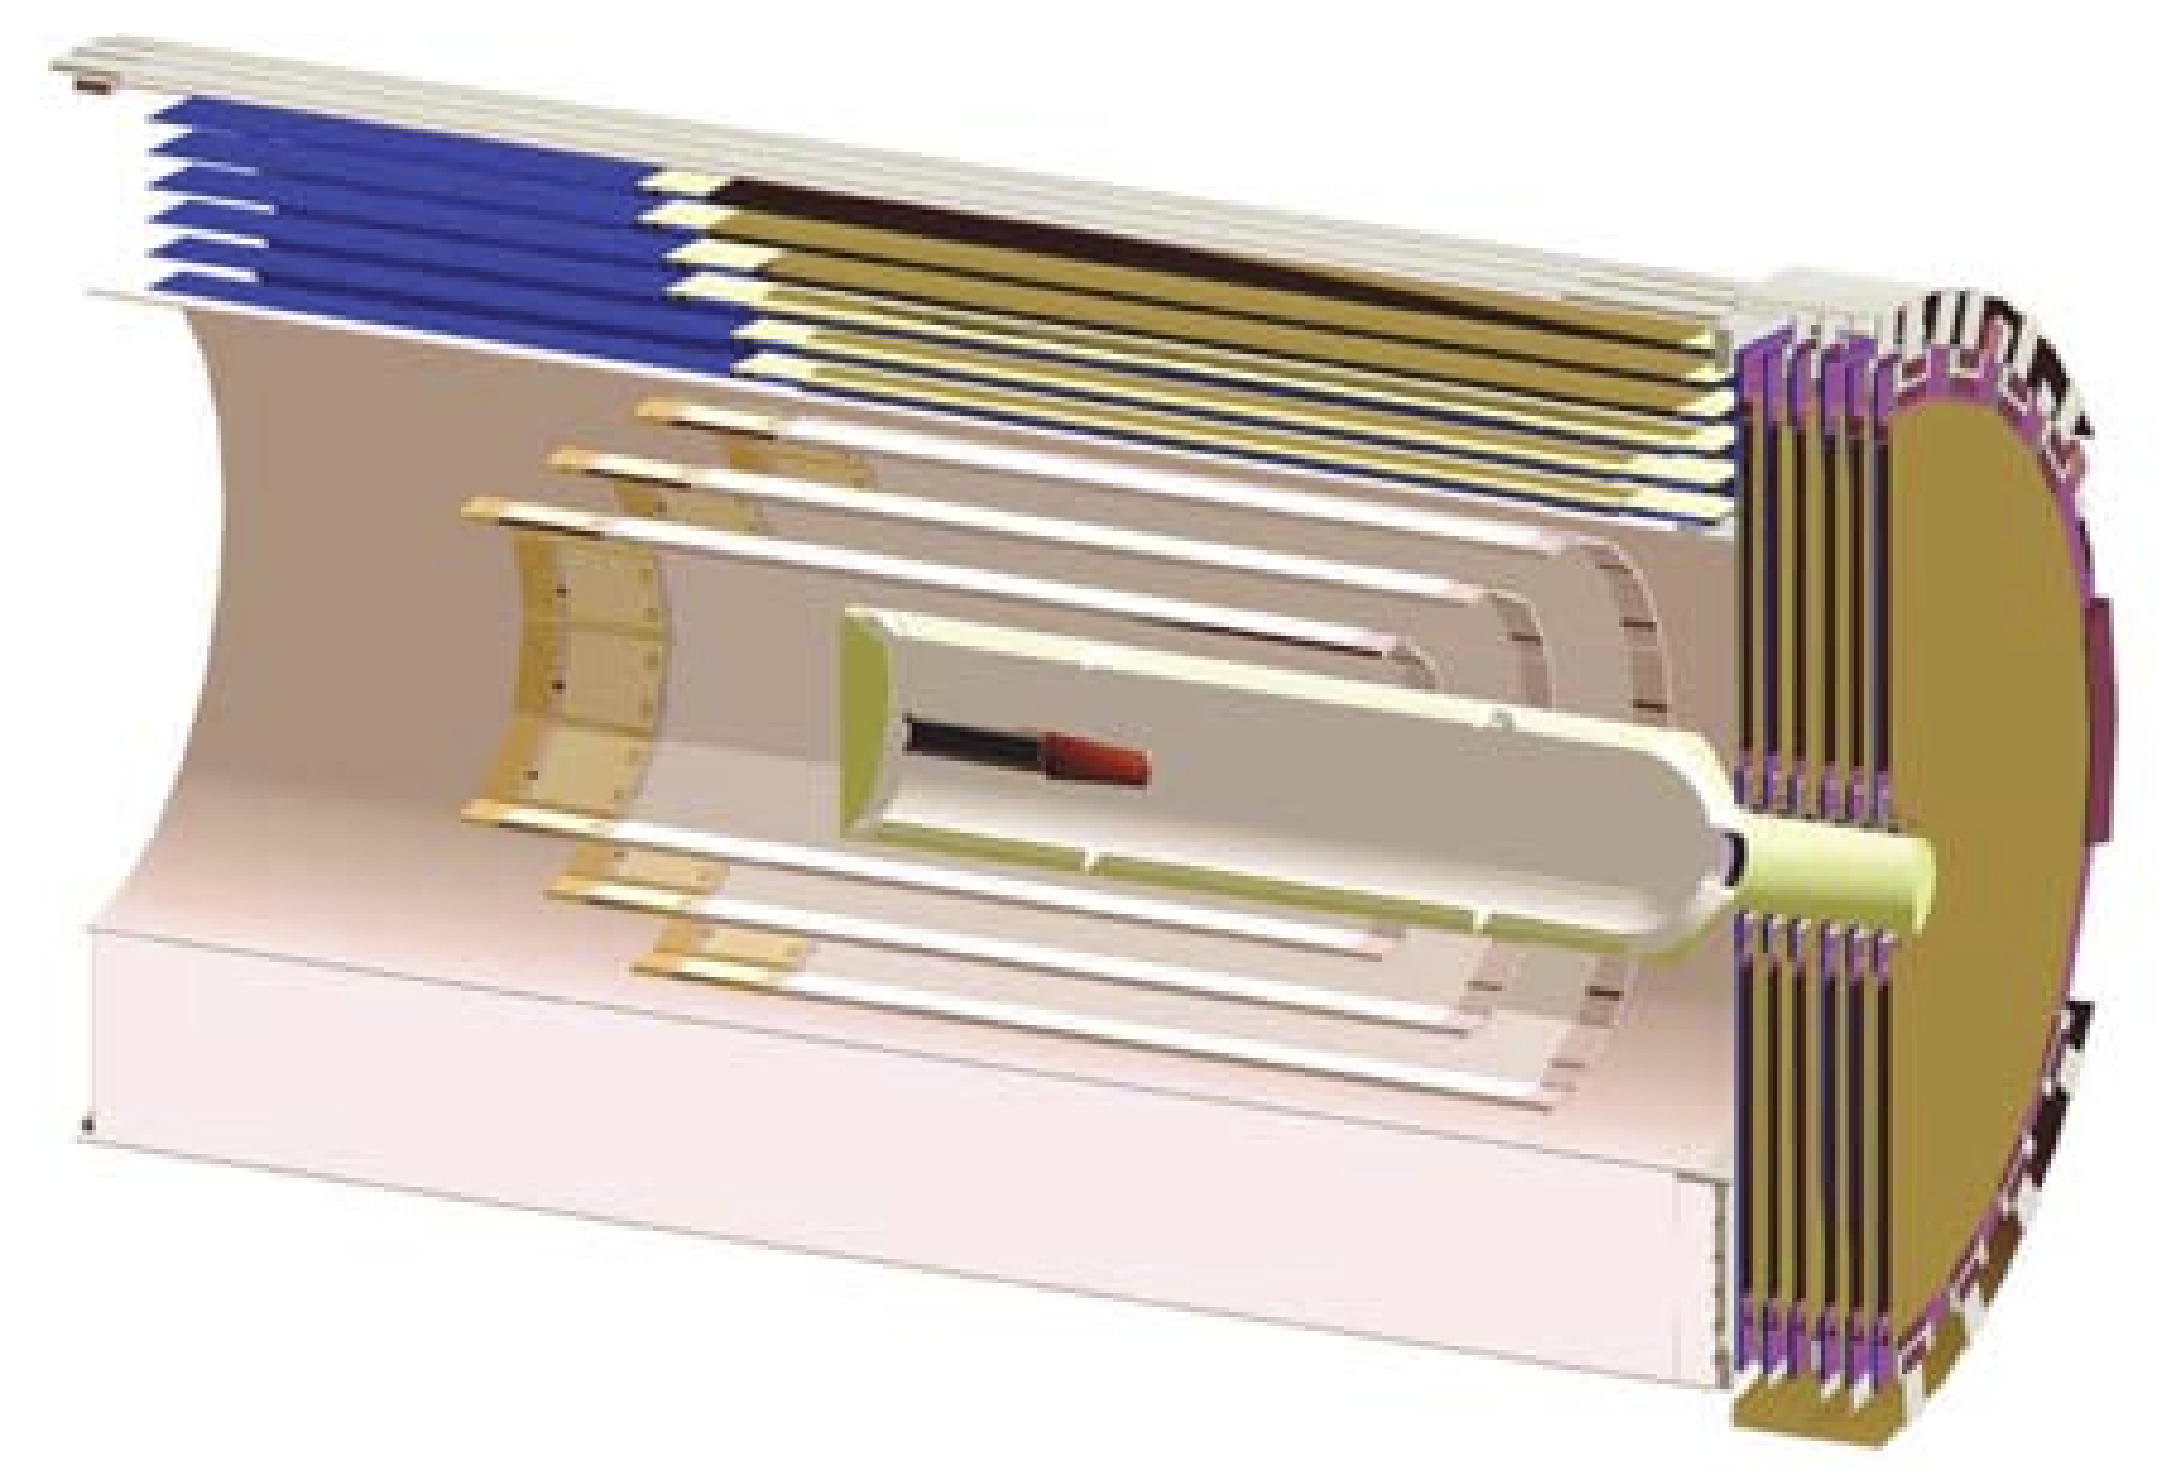
\includegraphics[width=0.3\textwidth]{Chapters/Ch2-Experiment/clas-12-exp/clas-detectors/cd/pics/CVT.png}\label{fig:mvt}
            }
            \hfill
            \subfloat[The CD, in retracted position for maintenance.]{
                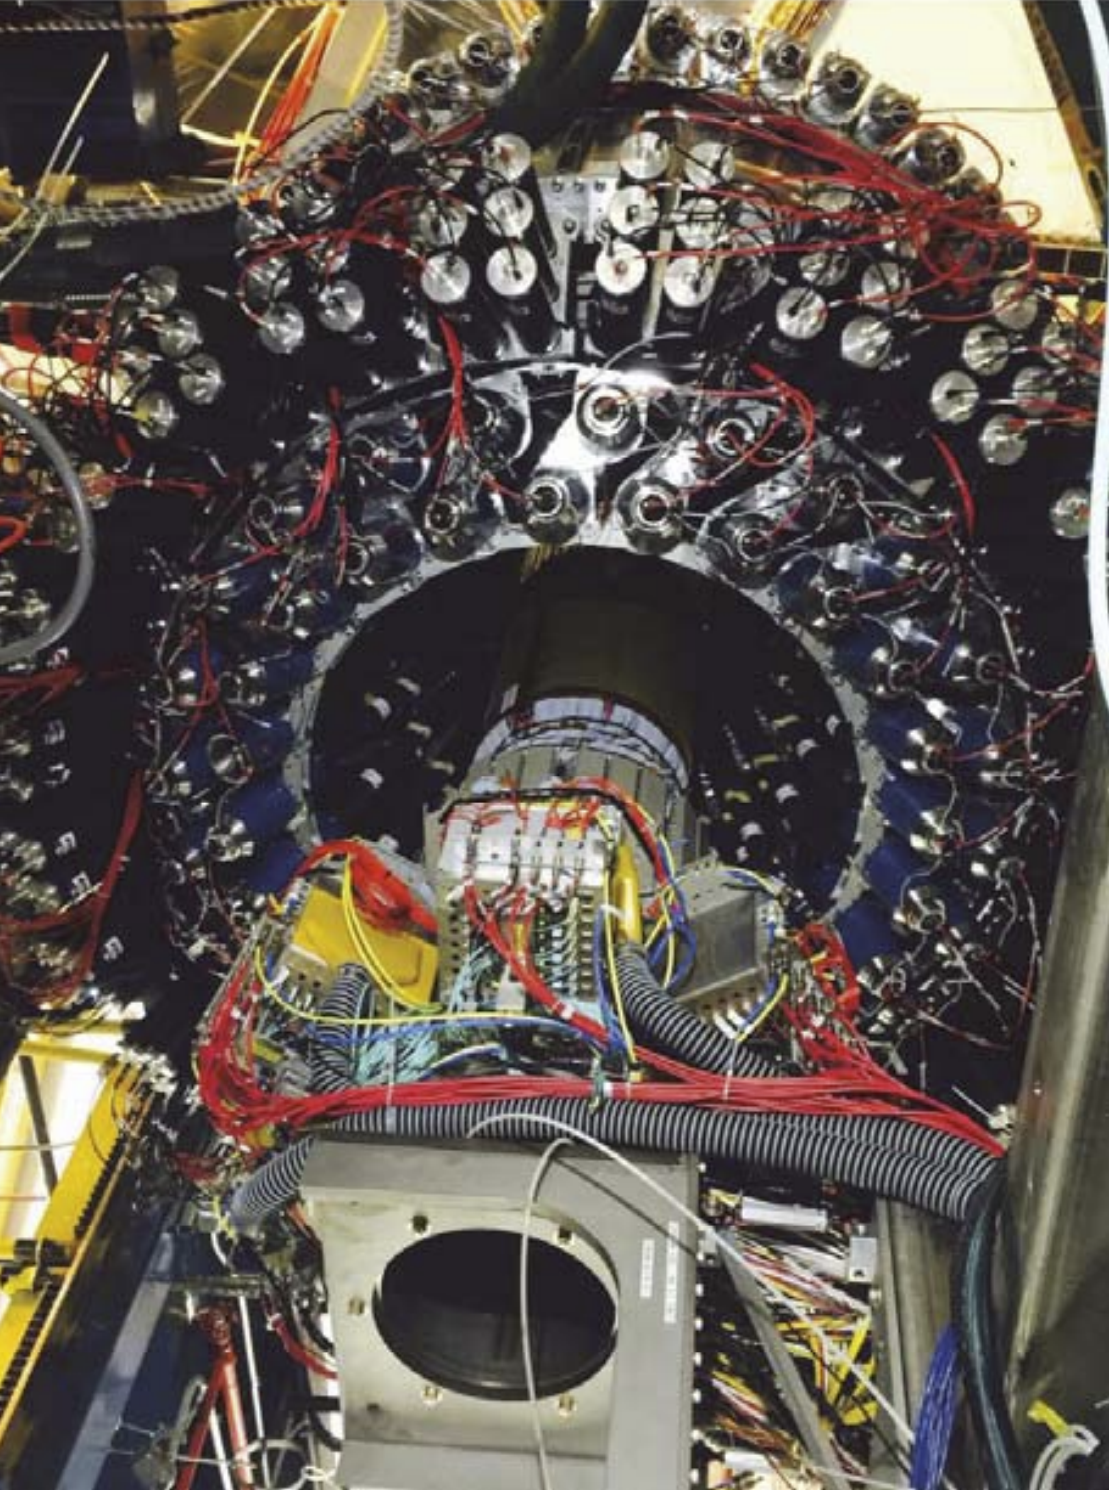
\includegraphics[trim={0 5cm 0 0},clip,width=0.3\textwidth]{Chapters/Ch2-Experiment/clas-12-exp/clas-detectors/cd/pics/real_CD.png}
            }
            \caption[Central Detector Packages]{Models of the CTOF (a) and CVT (b) and their physical realizations in the CD (c). Note the first three inner cylindrical layers of the CVT (b) correspond to the SVT, the outer six to the BMT, and the right end cap six to the FMT. Images from \parencite{Burkert2020TheLaboratory}.}
            \label{fig:your_labels}
        \end{figure}
     
        

\subsubsection*{Other System Components}

    At very low beam angles ($2.5^{\circ}$-$4.5^{\circ}$) there is the Forward Tagger (FT) \parencite{Acker2020TheTagger} which contains a tracker, homogeneous calorimeter, and hodoscope. At the other end of the beamline ($155^{\circ}$-$175^{\circ}$) there is the Backward Angle Neutron Detector (BAND)  \parencite{Segarra2020TheBAND}, which is not relevant for this analysis. Furthermore, the BAND and the Forward Micromegas Tracker (FMT)  \parencite{Acker2020TheTracker} were not installed at the time the data for this analysis was taken, although they have since been commissioned. 
    
    

\iffalse
%To possibly encorporate

    \begin{figure}[H]
        \centering
        \subfloat[]{
            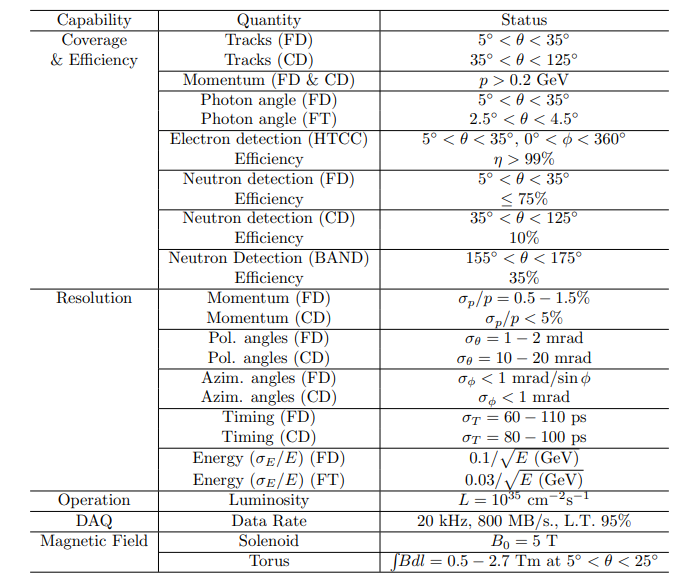
\includegraphics[width=0.3\textwidth]{Chapters/Ch2-Experiment/clas-12-exp/clas-detectors/other/pics/clas12-params.png}
        }
        \hfill
        \subfloat[]{
            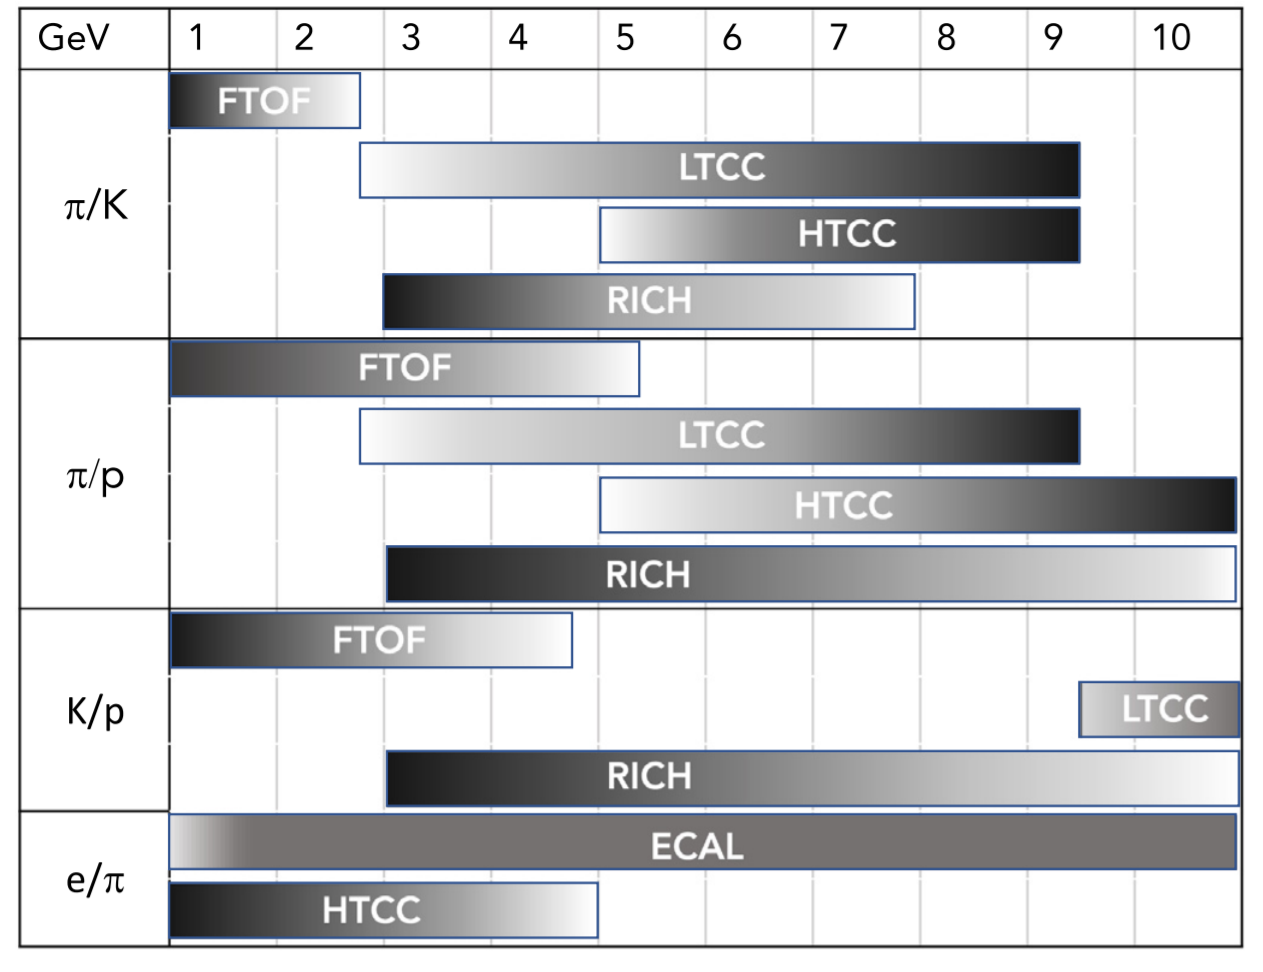
\includegraphics[width=0.3\textwidth]{Chapters/Ch2-Experiment/clas-12-exp/clas-detectors/other/pics/pid-clas12.png}
        }
        \hfill
        \subfloat[]{
            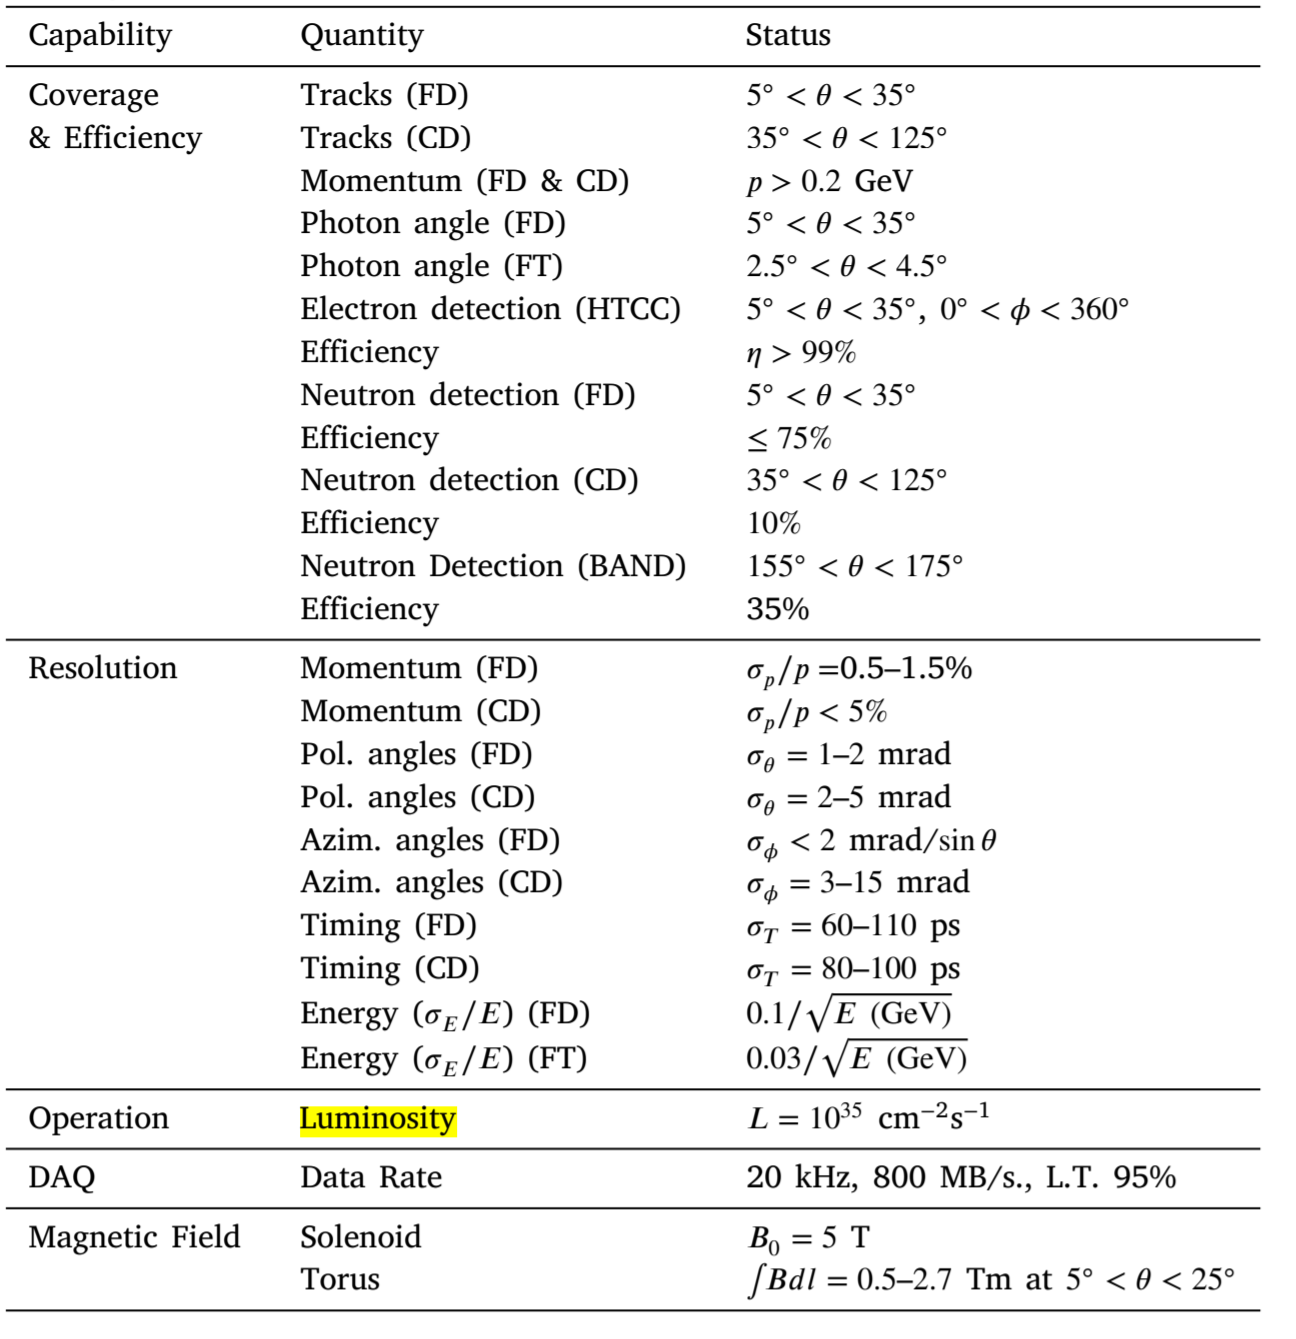
\includegraphics[width=0.3\textwidth]{Chapters/Ch2-Experiment/clas-12-exp/clas-detectors/other/pics/specs-v2-clas12.png}
        }
        \caption{Your caption goes here}
        \label{fig:others}
    \end{figure}

    
    %From sangbaek
    The Data Acquisition (DAQ) \parencite{Boyarinov2020TheSystem} dead-time can be corrected by using a gate at the FC that closes when the DAQ procedure is complete \parencite{Baltzell2020ThePerformance}. The total charge regardless of the gate is called the ungated charge, and the charge collected during the gate on is the gated charge. The ratio of the gated charge to the ungated charge is recorded as the DAQ live-time. The complete listing of detector components can be found in Table. 2.1. The CLAS12 detector components relevant to the particle 4-momentum vector reconstruction are grouped by their characteristics in Table. 2.2. The essential properties like threshold and resolutions and the prominent material components are also listed. 



    Table 2.2: The properties of the relevant subdetectors for the DVCS analysis. The
    properties relate mostly to the effective measurement uncertainties listed in each NIM
    article [135, 136, 140, 141, 143, 144, 147, 152].
    
    \begin{table}[ht]
        \centering
        \begin{tabularx}{\textwidth}{XccXX}
        \toprule
        Name & Coverage ($^\circ$) & Nominal Property & Material \\
        \midrule
        HTCC & 5-35 & $0.015 < p < 4.9$ GeV/c & CO$_2$ \\
        FTOF 1B & 5-35 & $60 - 110$ ps (t) & \\
        FTOF 1A & 5-35 & $90 - 180$ ps (t) & Plastic \\
        FTOF 2 & 35-45 & $170 - 180$ ps (t) & Scintillator \\
        CTOF & 35-125 & $80$ ps (t) & \\
        ECAL & 5-35 & $10\%/\sqrt{E}$ (E) & Pb (absorber) \\
        & & $1.2$ mrad ($\theta, \phi$) & Plastic scintillator \\
        FT-Cal & 2.5-4.5 & $2\%/\sqrt{E} \oplus 1\%$ (E) & PbWO$_4$ crystal \\
        & & $1.5\%$ ($\theta$) & \\
        & & $2^\circ$ ($\phi$) & \\
        DC & 5-40 & $1\%$ (p) & Aluminium wire \\
        & & $1$ mrad ($\theta$) & $90\%$ Ar \\
        & & $1$ mrad/sin $\theta$ ($\phi$) & $10\%$ CO$_2$ \\
        CVT & 35-125 & $5\%$ ($p_t$) & SVT: Si \\
        & & $10 - 20$ mrad ($\theta$) & BMT: $90\%$Ar + $10\%$C$_4$H$_{10}$ \\
        & & $5$ mrad ($\phi$) & \\
        FC & - & $0.48\%$ (L) & Pb \\
        \bottomrule
        \end{tabularx}
        \caption{Caption}
        \label{tab:my_label}
    \end{table}


\fi

